% Template for PLoS
% Version 3.4 January 2017
% -- FIGURES AND TABLES
%
% Please include tables/figure captions directly after the paragraph where they are first cited in the text.
%
% DO NOT INCLUDE GRAPHICS IN YOUR MANUSCRIPT
% - Figures should be uploaded separately from your manuscript file. 
% - Figures generated using LaTeX should be extracted and removed from the PDF before submission. 
% - Figures containing multiple panels/subfigures must be combined into one image file before submission.
% For figure citations, please use "Fig" instead of "Figure".
% See http://journals.plos.org/plosone/s/figures for PLOS figure guidelines.
%
% Tables should be cell-based and may not contain:
% - spacing/line breaks within cells to alter layout or alignment
% - do not nest tabular environments (no tabular environments within tabular environments)
% - no graphics or colored text (cell background color/shading OK)
% See http://journals.plos.org/plosone/s/tables for table guidelines.
%
% For tables that exceed the width of the text column, use the adjustwidth environment as illustrated in the example table in text below.
%
% % % % % % % % % % % % % % % % % % % % % % % %

\documentclass[10pt,letterpaper]{article}\usepackage[]{graphicx}\usepackage[]{color}
%% maxwidth is the original width if it is less than linewidth
%% otherwise use linewidth (to make sure the graphics do not exceed the margin)
\makeatletter
\def\maxwidth{ %
  \ifdim\Gin@nat@width>\linewidth
    \linewidth
  \else
    \Gin@nat@width
  \fi
}
\makeatother

\definecolor{fgcolor}{rgb}{0.345, 0.345, 0.345}
\newcommand{\hlnum}[1]{\textcolor[rgb]{0.686,0.059,0.569}{#1}}%
\newcommand{\hlstr}[1]{\textcolor[rgb]{0.192,0.494,0.8}{#1}}%
\newcommand{\hlcom}[1]{\textcolor[rgb]{0.678,0.584,0.686}{\textit{#1}}}%
\newcommand{\hlopt}[1]{\textcolor[rgb]{0,0,0}{#1}}%
\newcommand{\hlstd}[1]{\textcolor[rgb]{0.345,0.345,0.345}{#1}}%
\newcommand{\hlkwa}[1]{\textcolor[rgb]{0.161,0.373,0.58}{\textbf{#1}}}%
\newcommand{\hlkwb}[1]{\textcolor[rgb]{0.69,0.353,0.396}{#1}}%
\newcommand{\hlkwc}[1]{\textcolor[rgb]{0.333,0.667,0.333}{#1}}%
\newcommand{\hlkwd}[1]{\textcolor[rgb]{0.737,0.353,0.396}{\textbf{#1}}}%
\let\hlipl\hlkwb

\usepackage{framed}
\makeatletter
\newenvironment{kframe}{%
 \def\at@end@of@kframe{}%
 \ifinner\ifhmode%
  \def\at@end@of@kframe{\end{minipage}}%
  \begin{minipage}{\columnwidth}%
 \fi\fi%
 \def\FrameCommand##1{\hskip\@totalleftmargin \hskip-\fboxsep
 \colorbox{shadecolor}{##1}\hskip-\fboxsep
     % There is no \\@totalrightmargin, so:
     \hskip-\linewidth \hskip-\@totalleftmargin \hskip\columnwidth}%
 \MakeFramed {\advance\hsize-\width
   \@totalleftmargin\z@ \linewidth\hsize
   \@setminipage}}%
 {\par\unskip\endMakeFramed%
 \at@end@of@kframe}
\makeatother

\definecolor{shadecolor}{rgb}{.97, .97, .97}
\definecolor{messagecolor}{rgb}{0, 0, 0}
\definecolor{warningcolor}{rgb}{1, 0, 1}
\definecolor{errorcolor}{rgb}{1, 0, 0}
\newenvironment{knitrout}{}{} % an empty environment to be redefined in TeX

\usepackage{alltt}
\usepackage[top=0.85in,left=2.75in,footskip=0.75in]{geometry}

\usepackage{amsmath,amssymb}
\usepackage{changepage}
\usepackage[utf8x]{inputenc}
\usepackage{textcomp,marvosym}
\usepackage{cite}
\usepackage{nameref,hyperref}
\usepackage[right]{lineno}
\usepackage{microtype}
\DisableLigatures[f]{encoding = *, family = * }
\usepackage[table]{xcolor}
\usepackage{array}

% create "+" rule type for thick vertical lines
\newcolumntype{+}{!{\vrule width 2pt}}

% create \thickcline for thick horizontal lines of variable length
\newlength\savedwidth
\newcommand\thickcline[1]{%
  \noalign{\global\savedwidth\arrayrulewidth\global\arrayrulewidth 2pt}%
  \cline{#1}%
  \noalign{\vskip\arrayrulewidth}%
  \noalign{\global\arrayrulewidth\savedwidth}%
}

% \thickhline command for thick horizontal lines that span the table
\newcommand\thickhline{\noalign{\global\savedwidth\arrayrulewidth\global\arrayrulewidth 2pt}%
\hline
\noalign{\global\arrayrulewidth\savedwidth}}

% Remove comment for double spacing
%\usepackage{setspace} 
%\doublespacing

% Text layout
\raggedright
\setlength{\parindent}{0.5cm}
\textwidth 5.25in 
\textheight 8.75in

% Bold the 'Figure #' in the caption and separate it from the title/caption with a period
% Captions will be left justified
\usepackage[aboveskip=1pt,labelfont=bf,labelsep=period,justification=raggedright,singlelinecheck=off]{caption}
\renewcommand{\figurename}{Fig}

% Use the PLoS provided BiBTeX style
\bibliographystyle{plos2015}

% Remove brackets from numbering in List of References
\makeatletter
\renewcommand{\@biblabel}[1]{\quad#1.}
\makeatother

% Leave date blank
\date{}

% Header and Footer with logo
\usepackage{lastpage,fancyhdr,graphicx}
\usepackage{epstopdf}
\pagestyle{myheadings}
\pagestyle{fancy}
\fancyhf{}
\setlength{\headheight}{27.023pt}
\lhead{\includegraphics[width=2.0in]{PLOS-submission.eps}}
\rfoot{\thepage/\pageref{LastPage}}
\renewcommand{\footrule}{\hrule height 2pt \vspace{2mm}}
\fancyheadoffset[L]{2.25in}
\fancyfootoffset[L]{2.25in}
\lfoot{\sf PLOS}


\reversemarginpar
\usepackage[colorinlistoftodos]{todonotes}
%\usepackage[colorinlistoftodos,disable]{todonotes}

%% Include all macros below
\newcommand{\citationneeded}[2][]{\todo[color=blue, fancyline, #1]{\textbf{Citation Needed:} #2}}
\newcommand{\TODO}[2][]{\todo[color=red, fancyline, #1]{\textbf{TODO:} #2}}





\newcommand{\lorem}{{\bf LOREM}}
\newcommand{\ipsum}{{\bf IPSUM}}

%% END MACROS SECTION
\IfFileExists{upquote.sty}{\usepackage{upquote}}{}
\begin{document}
\vspace*{0.2in}

% Title must be 250 characters or less.
\begin{flushleft}
{\Large
\textbf\newline{Rethomics: an R framework to analyse high-throughput behavioural data} 
}
\newline
% Insert author names, affiliations and corresponding author email (do not include titles, positions, or degrees).
\\
Quentin Geissmann\textsuperscript{1*},
Luis G Rodriguez\textsuperscript{2},
Esteban J Beckwith\textsuperscript{1},
Giorgio F Gilestro\textsuperscript{1*}
\\
\bigskip
\textbf{1} Department of Life Sciences, Imperial College London, London, United Kingdom
\\
\textbf{2} Institute for Neuro- and Behavioral Biology, Westf{\"a}lische Wilhelms University, 48149 M{\"u}nster, Germany
\\
\bigskip


% Use the asterisk to denote corresponding authorship and provide email address in note below.
* qgeissmann@gmail.com, giorgio@gilest.ro

\end{flushleft}
% Please keep the abstract below 300 words
\section*{Abstract}
%Ethomics, a quantitative and high-throughput approach to animal behaviour, is a new and exciting field.
The recent development of automatised methods that can score various behaviours on a large number of animals
provides biologists with an unprecedented set of tools to decipher these complex phenotypes. 
Analysing such data comes with several challenges that are largely shared across acquisition platform and paradigms.
%However, there is little effort in providing a generic toolbox to specifically analyse multiple and long behavioural time series.
%To address this limitation, we developed the \texttt{rethomics} framework, 
%We present the \texttt{rethomics} framework, 
%a suite of \texttt{R} packages that altogether offers utilities to work through all data manipulation stage:
%import, store, analyse and visualise behavioural data.
In the article herein, we present \texttt{rethomics}, a set of \texttt{R} packages that unifies analysis of behavioural dataset in an efficient and flexible manner.
%We implemented it in \texttt{R}\cite{r_core_team_r:_2017} since it is widely taught and adopted by computational biologists.
%It is also complemented with a vast ecosystem of open-source packages.
\texttt{rethomics} offers a computational solution to store, manipulate and visualise large amounts of behavioural data.
We propose it as a tool to fill the gap between behavioural biology and data sciences, thus connecting computational and behavioural scientists.
Our software comes with a extensive documentation as well as a set of both practical and theoretical tutorials (available \href{https://rethomics.github.io}{https://rethomics.github.io}.

%In this article, we describe it and show an example of its application to the study of circadian rhythms and blooming field of sleep fruit flies.
%The \texttt{rethomics} framework is available and documented at \href{https://rethomics.github.io}{https://rethomics.github.io}.


\listoftodos

% Please keep the Author Summary between 150 and 200 words
% Use first person. PLOS ONE authors please skip this step. 
% Author Summary not valid for PLOS ONE submissions.   
%\section*{Author summary}

% TODO revert for sumbmisson
% \linenumbers
\TODO{revert line numbers before submission}
% TODO also embed bib

% Use "Eq" instead of "Equation" for equation citations.
\section*{Introduction}
The behaviour of an animal is a complex phenotypical manifestation of the interaction between its nervous system, internal state and environment.
In the last few decades, our ability to record vast quantities of various phenotypical data has tremendously increased\cite{stephens_big_2015}.
The scoring of behaviours is certainly not an exception to this trend \cite{reiser_ethomics_2009}.
Indeed, many platforms have been developed in order to allow biologists to continuously record behaviours such as activity\cite{faville_how_2015}, position\cite{pelkowski_novel_2011} and feeding\cite{itskov_automated_2014,ro_flic:_2014} of single or multiple\cite{swierczek_high-throughput_2011,perez-escudero_idtracker:_2014} animals over long durations (days or weeks).

The availability of large amounts of data paves the way for in-depth quantitative analyses which, in turn, leads to the characterisation of new principles
and ultimately a better understanding of their underlying biology\cite{brown_study_2017,berman_measuring_2018}.
The multiplicity of model organisms, hypotheses and paradigms makes the existence of a diverse set of recording tools important.
However, when it comes to the subsequent processing of the results, there is no unified, programmatic, framework that could be used as a palette of building blocks in a pipeline.

Scripting interfaces are the standard in data sciences and statistics since they help delivering reproducible results \cite{peng_reproducible_2011,stodden_toward_2013}.
In addition such tools can be used on remote resources such as computer clusters, which makes them more scalable to the context of `big data'\cite{hashem_rise_2015}.
For example, the field of bioinformatics benefits from sharing standard files formats, modular command line tools\cite{roumpeka_review_2017} and software packages\cite{huber_orchestrating_2015} that can be assembled to build pipelines\cite{leipzig_review_2017}.
Since many aspect of behaviour analysis are are becoming increasingly linked to data sciences, the development of common tools and data structures would be an interesting resource to the community.
Behavioural experiments result in sets of long time series (sometimes multivariate and irregular), the data, but also involve a formal description of the treatment applied to each individual.
Such implicit structure is consistent between acquisition platforms and experimental paradigms, which broaden the scope for developing of utilities an shared principles.

In the article herein, we describe the \texttt{rethomics} platform, a collection of packages offering a solution to import, store, manipulate and visualise large amounts of behavioural data.
We also present two examples of application: the analysis of circadian rhythm in fruit flies.


\section*{Design and Implementation}
\texttt{rethomics} is implemented in \texttt{R}\cite{r_core_team_r:_2017}, since it is widely taught and adopted by computational biologists,
as a collection of packages related to one another (Fig~\ref{fig:fig-1}).

This architecture paradigm follows the model of modern frameworks such as the \texttt{tidyverse}\cite{wickham_tidyverse:_2017}, which results in increased testability and maintainability.
In it, the different tasks of the analysis workflow (\emph{i.e.} data import, manipulation and visualisation)
are explicitly handled by different packages.
At the core of \texttt{rethomics}, the \texttt{behavr} package offers a very flexible and efficient solution to store large amounts data (\emph{e.g.} position and activity) as well as metadata (\emph{e.g.} treatment and genotype) in a single \texttt{data.table}-derived object\cite{dowle_data.table:_2017}.
Any input package will import experimental data as a \texttt{behavr} table which can, in turn, be analysed and visualised regardless of the original input platform.
Results and plots integrate seamlessly into the \texttt{R} ecosystem, hence providing users with state-of-the-art visualisation and statistical tools.

% Place figure captions after the first paragraph in which they are cited.



\begin{figure}[!h]
%	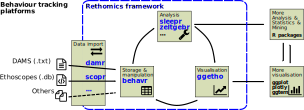
\includegraphics[width=1\textwidth]{fig/fig-1.pdf}
	\caption{{\bf The \texttt{rethomics} workflow.}
		Diagram representing the interplay between, from left to right, the raw data, the \texttt{rethomics} packages (in blue) and the rest of the \texttt{R} ecosystem.}
	\label{fig:fig-1}
\end{figure}


\subsection*{Internal data structure}
We created \texttt{behavr} (Fig~\ref{fig:fig-2}A), a new data structure, based on the widely adopted \texttt{data.table} object, in order to address two challenges that are inherent to handling ethomics results.

Firstly, there could be very long (typically $k_i > 10^8, \forall i \in [1,n]$), multivariate (often, $q > 10$), time series for each individual.
For instance, each series could represent variables that encode coordinates, orientation, dimensions, activity, colour intensity and so on, sampled several times per second, over multiple days.
Therefore, the data structure must be computationally efficient -- both in term of memory footprint and processing speed. 

Secondly, a large number of individuals are often studied (typically $n > 100$).
Each individual ($i$) is associated with metadata: a set of $p$ ``metavariables'' that describe experimental conditions.
For instance, metadata stores information regarding the date and location of the experiment, treatment, genotype, sex, \emph{post hoc} observations and other arbitrary metavariables.
It is interesting to record multiple metavariables since they can later be used as covariates. 
Therefore, typically $p > 10$.

\texttt{behavr} tables link metadata and data within the same object, extending the syntax of \texttt{data.table} to manipulate, join and access metadata (Fig~\ref{fig:fig-2}B).
This approach guarantees that any data point can be mapped correctly to its parent metadata.
It also allows implicit update of metadata when data is altered.
For instance, when is data filtered, only the remaining individuals should be in the new metadata. 
It is also important that metadata and data can interoperate.
For instance, when one wants to update a variable according to the value of a metavariable (say, alter the variable $x$ only for animals with the metavariable $sex=``male"$). The online tutorials and documentation provide a detailed set of examples and concrete use cases of \texttt{behavr}. 


\begin{figure}[!h]
% 	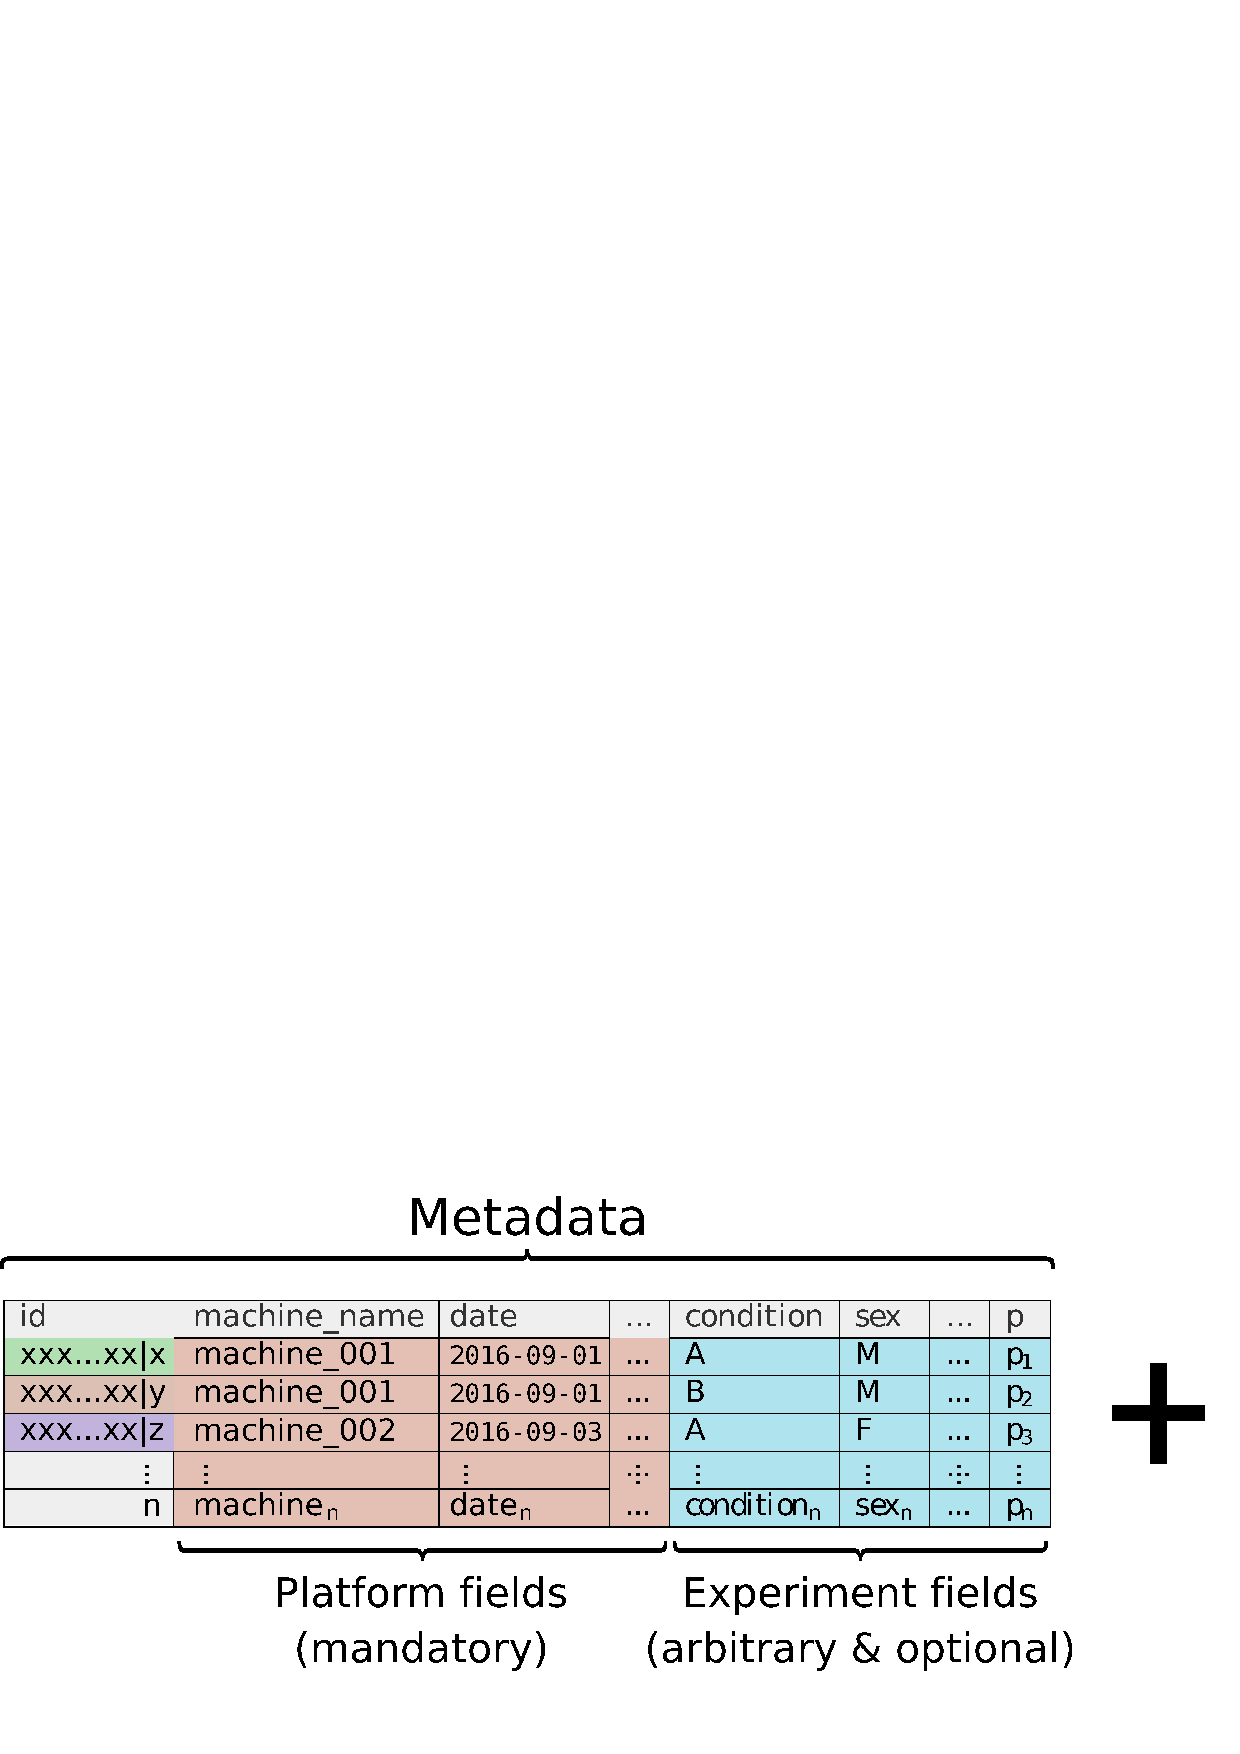
\includegraphics[width=1\textwidth]{fig/fig-2.pdf}
	\caption{{\bf \texttt{behavr} table.}
	A: Illustration of a \texttt{behavr} object, the core data structure in \texttt{rethomics}.
		The metadata holds a single row for each of the $n$ individuals. 
		Its columns, the $p$ metavariables, are one of two kinds: either required -- and defined by the acquisition platform (\emph{i.e.} used to fetch the data) -- or user-defined (\emph{i.e.} arbitrary).
		In the data, each row is a ``read'' (\emph{i.e.} information about one individual at one time-point).
		It is formed of $q$ variables and is expected to have a very large number of reads, $k$, for each individual $i$.
		Data and metadata are implicitly joined on the \texttt{id} field.
		Note that the names used in this for variables and metavariable in this example are only plausible cases which will likely differ in practice. 
		B: Non exhaustive list of uses of a \texttt{behavr} table (referred as \texttt{dt}). 
		In addition to operations on data, which are inherited from \texttt{data.table},
		we provide utilities designed specifically to act on both metadata and data.  
		Commented examples are prefixed by \texttt{>}.
	}
	\label{fig:fig-2}
\end{figure}

\subsection*{Data import}
Data import packages translate results from a recording platform (\emph{e.g.} text files and databases) into a single \texttt{behavr} object.
Currently, we provide a package to read single or multi-beam Drosophila Activity Monitor System (Trikinetics Inc.) data and another one for Ethoscope data\cite{geissmann_ethoscopes:_2017}.
Although the structure of the raw results is very different, conceptually, loading data is very similar.
In all cases, the user is asked to generate a metadata table (one row per individual). 
In it, there will be both mandatory and optional columns.
The mandatory ones are the necessary and sufficient information to fetch data (\emph{e.g.} machine id, region of interest and date). 
The optional columns are user-defined arbitrary fields that translate experimental conditions (\emph{e.g.} treatment, genotype and sex).

In this respect, the metadata file is a standardised and comprehensive data frame describing an experiment.
It explicitly lists all treatments and individuals, which facilitates interspersion of conditions (indeed, without it, users are tempted to simplify their experimental design by, for instance, confounding device/location and treatment).
Furthermore, it streamlines the inclusion and analysis of further replicates in the same workflow.
Indeed, additional replicates can simply be added as new rows -- and the ID of the replicate later used, if needed, as a covariate.	


\subsection*{Visualisation}
Long time series often need to be preprocessed before visualisation.
Typically, users are interested in understanding individual or population trends over time.
To integrate visualisation in \texttt{rethomics}, we implemented \texttt{ggetho},
a package that offers new tools that extent the widely adopted \texttt{ggplot2}\cite{wickham_ggplot2:_2016}.
It provides preprocessing utilities as well as new layers and scales.
Our tools make full use of the internal \texttt{behavr} structure to deliver efficient representations of temporal trends.
It particularly applies to the visualisation of long experiments, with the ability to, for instance, display ``double-plotted actograms'', periodograms, annotate light and dark phases and wrap time over a given period. 
Importantly, \texttt{ggetho} is fully compatible with \texttt{ggplot2}.

\subsection*{Circadian and sleep analysis}
The packages \texttt{zeitgebr} and \texttt{sleepr} provide tools to analyse circadian behaviours and sleep, respectively.
Together, they offer a suite of methods to compute autocorrelogram, $\chi{}^2$\cite{sokolove_chi_1978} and Lomb-Scargle\cite{ruf_lomb-scargle_1999}
periodograms and find their peaks, score sleep from inactivity (\emph{i.e.} using the ``five-minute rule''), and characterise the architecture of sleep bouts (\emph{e.g.} number, length and latency).







\section*{Results}
In order to illustrate the workflow of \texttt{rethomics}, we provide a straightforward and simplified example which could be readily modified for more intricate cases. 

The study of circadian rhythm, employing fruit flies as an animal model, is a well established research field recently awarded with the Nobel Prize in Physiology or Medicine.
Importantly, DAM2 (the second, and most popular, version of the Drosophila Activity Monitors System) is the most widely adopted behaviour recording platform in this research field.
We gathered a subset of the data from a recent publication\cite{buhl_quasimodo_2016}, which was graciously made publicly available by the authors\cite{ogueta_ll_2018}.
Wild type flies are highly rhythmic in Light-Dark (LD) cycles and become arrhythmic in constant light (LL).
In their study, the authors gain understanding of the function of the molecular clock by showing that overexpression of the gene NKCC makes the flies rhythmic in both LD and LL,
and that the endogenous period in LL is longer than 24 hours.

We took two genotypes employed in the study, one control group (NKCC\textsuperscript{ox}/+) and one where NKCC\textsuperscript{ox} is overexpressed in all clock neurons (TIM/NKCC\textsuperscript{ox}).
In particular, we re-analysed two repetitions of the same experiment in which a total of 58 animals were recorded for three to four days in LD and then subjected to constant light for six days.
The \texttt{metadata.csv} file, which describes exhaustively all individuals, as well as all the associated result files can be downloaded at \href{https://zenodo.org/record/1172980}{https://zenodo.org/record/1172980}.
As a prerequisite, we downloaded the data, extracted the zip archive in our working directory.
We start the analysis by loading the necessary rethomics packages (see availability section for installation instructions):

\begin{knitrout}
\definecolor{shadecolor}{rgb}{0.969, 0.969, 0.969}\color{fgcolor}\begin{kframe}
\begin{alltt}
\hlkwd{library}\hlstd{(damr)}      \hlcom{# input DAM data}
\hlkwd{library}\hlstd{(zeitgebr)}  \hlcom{# periodogram computation}
\hlkwd{library}\hlstd{(sleepr)}    \hlcom{# sleep analysis}
\hlkwd{library}\hlstd{(ggetho)}    \hlcom{# behaviour visualisation}
\end{alltt}
\end{kframe}
\end{knitrout}

Then, the metadata file is read and linked to the \texttt{.txt} result files.

\begin{knitrout}
\definecolor{shadecolor}{rgb}{0.969, 0.969, 0.969}\color{fgcolor}\begin{kframe}
\begin{alltt}
\hlstd{metadata} \hlkwb{<-} \hlkwd{link_dam_metadata}\hlstd{(}\hlstr{"metadata.csv"}\hlstd{,} \hlstr{"."}\hlstd{)}   \hlcom{# linking}
\end{alltt}


{\ttfamily\noindent\bfseries\color{errorcolor}{\#\# Error in link\_dam\_metadata("{}metadata.csv"{}, "{}."{}): could not find function "{}link\_dam\_metadata"{}}}\begin{alltt}
\hlcom{# print(metadata)                                     # check metadata}
\hlstd{dt} \hlkwb{<-} \hlkwd{load_dam}\hlstd{(metadata)}                             \hlcom{# loading}
\end{alltt}


{\ttfamily\noindent\bfseries\color{errorcolor}{\#\# Error in load\_dam(metadata): could not find function "{}load\_dam"{}}}\begin{alltt}
\hlkwd{summary}\hlstd{(dt)}                                           \hlcom{# quick summary}
\end{alltt}


{\ttfamily\noindent\bfseries\color{errorcolor}{\#\# Error in object[[i]]: object of type 'closure' is not subsettable}}\end{kframe}
\end{knitrout}

\subsection*{Preprocessing}
The two replicates do not have the same baseline time and we would like to express the time relative to the important event:
the transition from LD to LL. 
Therefore, we subtract the \texttt{baseline\_days} metavariable from the \texttt{t} variable.
This gives us an opportunity to illustrate the use \texttt{xmv()}, which expands metavariables as variables.
In addition, we use the \texttt{data.table} syntax to create, in place, a \texttt{moving} variable.
It is \texttt{TRUE} when and only when \texttt{activity} is greater than zero:

\begin{knitrout}
\definecolor{shadecolor}{rgb}{0.969, 0.969, 0.969}\color{fgcolor}\begin{kframe}
\begin{alltt}
\hlcom{# baseline subtraction -- note the use of xmv}
\hlstd{dt[,t} \hlkwb{:=} \hlstd{t} \hlopt{-} \hlkwd{days}\hlstd{(}\hlkwd{xmv}\hlstd{(baseline_days))]}
\hlstd{dt[, moving} \hlkwb{:=}  \hlstd{activity} \hlopt{>} \hlnum{0}\hlstd{]}
\end{alltt}
\end{kframe}
\end{knitrout}

\begin{knitrout}
\definecolor{shadecolor}{rgb}{0.969, 0.969, 0.969}\color{fgcolor}\begin{kframe}
\begin{alltt}
\hlkwd{summary}\hlstd{(dt)}
\end{alltt}
\begin{verbatim}
## behavr table with:
##  58	individuals
##  8	metavariables
##  3	variables
##  1.58722e+05	measurements
##  1	key (id)
\end{verbatim}
\end{kframe}
\end{knitrout}

To simplify visualisation, we create our own \texttt{label} metavariable, as the combination of a number and \texttt{genotype}.
In the restricted context of this analysis, \texttt{label} acts as a unique identifier.
Importantly, we keep \texttt{id}, which is more rigorous and universal.



\begin{knitrout}
\definecolor{shadecolor}{rgb}{0.969, 0.969, 0.969}\color{fgcolor}\begin{kframe}
\begin{alltt}
\hlstd{dt[, label} \hlkwb{:=} \hlkwd{interaction}\hlstd{(}\hlnum{1}\hlopt{:}\hlstd{.N, genotype),} \hlkwc{meta} \hlstd{= T]}
\hlkwd{print}\hlstd{(dt)}
\end{alltt}
\end{kframe}
\end{knitrout}


\subsection*{Curation}
It is important to visualise an overview of how each individual behaved and, if necessary, alter the data accordingly. For this, we generate a tile plot (Fig~\ref{fig:fig-3}A).

\begin{figure}[!h]
%    \includegraphics[width=1\textwidth]{fig/fig-3.pdf}
	\caption{{\bf Experiment quality control.}
			Tile plot showing the fraction of time spent moving as a colour intensity.
			Each individual is represented by a row and time, on the x-axis, is binned in 30 minutes.
			A: Uncurated raw data.
			B: Data after the curation step. Time was trimmed and data from dead animals removed. 
			Red `\textbf{+}' symbols show animals that were removed from the subsequent analysis as they had less than five complete days in LL.}
	\label{fig:fig-3}
\end{figure}

\begin{knitrout}
\definecolor{shadecolor}{rgb}{0.969, 0.969, 0.969}\color{fgcolor}\begin{kframe}
\begin{alltt}
\hlcom{# make a ggplot object with label on the y and moving on the z axis}
\hlstd{fig3A} \hlkwb{<-} \hlkwd{ggetho}\hlstd{(dt,} \hlkwd{aes}\hlstd{(}\hlkwc{y} \hlstd{= label,} \hlkwc{z} \hlstd{= moving))} \hlopt{+}
  \hlcom{# show data as a tile plot}
  \hlcom{# that is z is a pixel whose intensity maps moving}
  \hlkwd{stat_tile_etho}\hlstd{()} \hlopt{+}
  \hlcom{# add layers to draw annotations to show L and D phases}
  \hlcom{# as white and black, respectively}
  \hlcom{# the first layer is for the baseline (until t = 0)}
  \hlkwd{stat_ld_annotations}\hlstd{(}\hlkwc{x_limits} \hlstd{=} \hlkwd{c}\hlstd{(dt[,}\hlkwd{min}\hlstd{(t)],} \hlnum{0}\hlstd{))} \hlopt{+}
  \hlcom{# in the 2nd one, we start at 0 and use grey }
  \hlcom{# instead of black as we work in LL}
  \hlkwd{stat_ld_annotations}\hlstd{(}\hlkwc{x_limits} \hlstd{=} \hlkwd{c}\hlstd{(}\hlnum{0}\hlstd{, dt[,} \hlkwd{max}\hlstd{(t)]),}
                      \hlkwc{ld_colours} \hlstd{=} \hlkwd{c}\hlstd{(}\hlstr{"white"}\hlstd{,} \hlstr{"grey"}\hlstd{))}
\end{alltt}
\end{kframe}
\end{knitrout}


The activity of dead or escaped animals is falsely scored as long series of zeros (see, for instance, individual 30 and 18 in Fig~\ref{fig:fig-3}A).
Our \texttt{sleepr} package offers a tool to detect and remove such artefactual data.

\begin{knitrout}
\definecolor{shadecolor}{rgb}{0.969, 0.969, 0.969}\color{fgcolor}\begin{kframe}
\begin{alltt}
\hlcom{# remove data after death}
\hlstd{dt} \hlkwb{<-} \hlstd{sleepr}\hlopt{::}\hlkwd{curate_dead_animals}\hlstd{(dt, moving)}
\end{alltt}
\end{kframe}
\end{knitrout}


In addition, we can trim our data to have the same number of days across experiments and individuals.
\begin{knitrout}
\definecolor{shadecolor}{rgb}{0.969, 0.969, 0.969}\color{fgcolor}\begin{kframe}
\begin{alltt}
\hlcom{# filter dt between -2d and 6d}
\hlstd{dt} \hlkwb{<-} \hlstd{dt[t} \hlopt \hlkwd{days}\hlstd{(}\hlkwd{c}\hlstd{(}\hlopt{-}\hlnum{2}\hlstd{,} \hlnum{6}\hlstd{))]}
\hlcom{# same as above}
\hlstd{fig3B} \hlkwb{<-} \hlkwd{ggetho}\hlstd{(dt,} \hlkwd{aes}\hlstd{(}\hlkwc{y} \hlstd{= label,} \hlkwc{z} \hlstd{= moving))} \hlopt{+}
    \hlkwd{stat_tile_etho}\hlstd{()} \hlopt{+}
    \hlkwd{stat_ld_annotations}\hlstd{(}\hlkwc{x_limits} \hlstd{=} \hlkwd{c}\hlstd{(dt[,} \hlkwd{min}\hlstd{(t)],} \hlnum{0}\hlstd{))} \hlopt{+}
    \hlkwd{stat_ld_annotations}\hlstd{(}\hlkwc{x_limits} \hlstd{=} \hlkwd{c}\hlstd{(}\hlnum{0}\hlstd{, dt[,} \hlkwd{max}\hlstd{(t)]),}
                        \hlkwc{ld_colours} \hlstd{=} \hlkwd{c}\hlstd{(}\hlstr{"white"}\hlstd{,} \hlstr{"grey"}\hlstd{))}
\end{alltt}
\end{kframe}
\end{knitrout}

For the purpose of this example, we also exclude animals that died prematurely, and keep only individuals that have \emph{at least five days in LL}. An overview of the curate data can be visualised in Fig~\ref{fig:fig-3}B.



\begin{knitrout}
\definecolor{shadecolor}{rgb}{0.969, 0.969, 0.969}\color{fgcolor}\begin{kframe}
\begin{alltt}
\hlcom{# for each id, we check for validity}
\hlstd{valid_dt} \hlkwb{<-} \hlstd{dt[,} \hlkwd{.}\hlstd{(}\hlkwc{valid} \hlstd{=} \hlkwd{max}\hlstd{(t)} \hlopt{>} \hlkwd{days}\hlstd{(}\hlnum{5}\hlstd{)),} \hlkwc{by} \hlstd{= id]}
\hlcom{# a vector of all valid ids}
\hlstd{valid_ids} \hlkwb{<-} \hlstd{valid_dt[valid} \hlopt{==} \hlstd{T, id]}
\hlcom{# filter dt with the valid ids}
\hlstd{dt} \hlkwb{<-} \hlstd{dt[id} \hlopt \hlstd{valid_ids]}
\hlkwd{summary}\hlstd{(dt)}
\end{alltt}
\begin{verbatim}
## behavr table with:
##  52	individuals
##  9	metavariables
##  3	variables
##  1.19546e+05	measurements
##  1	key (id)
\end{verbatim}
\end{kframe}
\end{knitrout}

Note that as a result, we now have 52 ``valid''individuals.


\subsection*{Double-plotted actograms}
``Double-plotted actograms'' are a common visualisation of periodicity and rhythmicity in circadian experiments.
In  \nameref{S1-Fig}A, we show the double-plotted actograms of each animal.
A representative sample of four individuals for each genotype is shown in Fig~\ref{fig:fig-4}A.

\begin{knitrout}
\definecolor{shadecolor}{rgb}{0.969, 0.969, 0.969}\color{fgcolor}\begin{kframe}
\begin{alltt}
\hlcom{# we also show a subset of this figure in 4A}
\hlstd{figS1A} \hlkwb{<-} \hlkwd{ggetho}\hlstd{(dt,} \hlkwd{aes}\hlstd{(}\hlkwc{z} \hlstd{= moving),} \hlkwc{multiplot} \hlstd{=} \hlnum{2}\hlstd{)} \hlopt{+}
            \hlcom{# bars n the z axis could }
            \hlcom{# one could also use stat_tile_etho}
            \hlkwd{stat_bar_tile_etho}\hlstd{()} \hlopt{+}
            \hlcom{# split plot by individual}
            \hlkwd{facet_wrap}\hlstd{(} \hlopt{~} \hlstd{label,} \hlkwc{ncol} \hlstd{=} \hlnum{4}\hlstd{)} \hlopt{+}
            \hlcom{# rename the y axis}
            \hlkwd{scale_y_discrete}\hlstd{(}\hlkwc{name} \hlstd{=} \hlstr{"Day"}\hlstd{)}
\end{alltt}
\end{kframe}
\end{knitrout}




\subsection*{Periodograms}
Ultimately, in order to quantify periodicity and rhythmicity, we compute periodograms.
Several methods are implemented in \texttt{zeitbebr}: $\chi{}^2$, Lomb-Scargle, autocorrelation 
and Fourier.
In this example, we generate $\chi{}^2$ periodograms and lay them out in a grid.
Periodograms for the subset of eight animals used in Fig~\ref{fig:fig-4}A is shown in Fig~\ref{fig:fig-4}B. 
See \nameref{S1-Fig}B for the visualisation of all individuals.

\begin{knitrout}
\definecolor{shadecolor}{rgb}{0.969, 0.969, 0.969}\color{fgcolor}\begin{kframe}
\begin{alltt}
\hlcom{# only the LL data}
\hlstd{dt_ll} \hlkwb{<-} \hlstd{dt[t} \hlopt{>} \hlkwd{days}\hlstd{(}\hlnum{1}\hlstd{)]}
\hlcom{# compute chi sqr periodogram }
\hlstd{per_dt} \hlkwb{<-} \hlkwd{periodogram}\hlstd{(moving,}
                        \hlstd{dt_ll,}
                        \hlkwc{resample_rate} \hlstd{=} \hlnum{1} \hlopt{/} \hlkwd{mins}\hlstd{(}\hlnum{10}\hlstd{),}
                        \hlkwc{FUN}\hlstd{=chi_sq_periodogram)}

\hlstd{per_dt} \hlkwb{<-} \hlkwd{find_peaks}\hlstd{(per_dt)}
\hlcom{# we also show a subset of this figure in supplementary materials}
\hlstd{figS1B} \hlkwb{<-} \hlkwd{ggperio}\hlstd{(per_dt,} \hlkwd{aes}\hlstd{(}\hlkwc{y} \hlstd{= power,} \hlkwc{peak} \hlstd{= peak))} \hlopt{+}
                  \hlcom{# periododogram drawn as a line}
                  \hlkwd{geom_line}\hlstd{()} \hlopt{+}
                  \hlcom{# the significance line in red}
                  \hlkwd{geom_line}\hlstd{(}\hlkwd{aes}\hlstd{(}\hlkwc{y} \hlstd{= signif_threshold),} \hlkwc{colour} \hlstd{=} \hlstr{"red"}\hlstd{)} \hlopt{+}
                  \hlcom{# point and text at the peak}
                  \hlkwd{geom_peak}\hlstd{()} \hlopt{+}
                  \hlcom{# divide plot by individual}
                  \hlkwd{facet_wrap}\hlstd{(} \hlopt{~} \hlstd{label,} \hlkwc{ncol} \hlstd{=} \hlnum{4}\hlstd{)}
\end{alltt}
\end{kframe}
\end{knitrout}







\begin{figure}[!h]
%	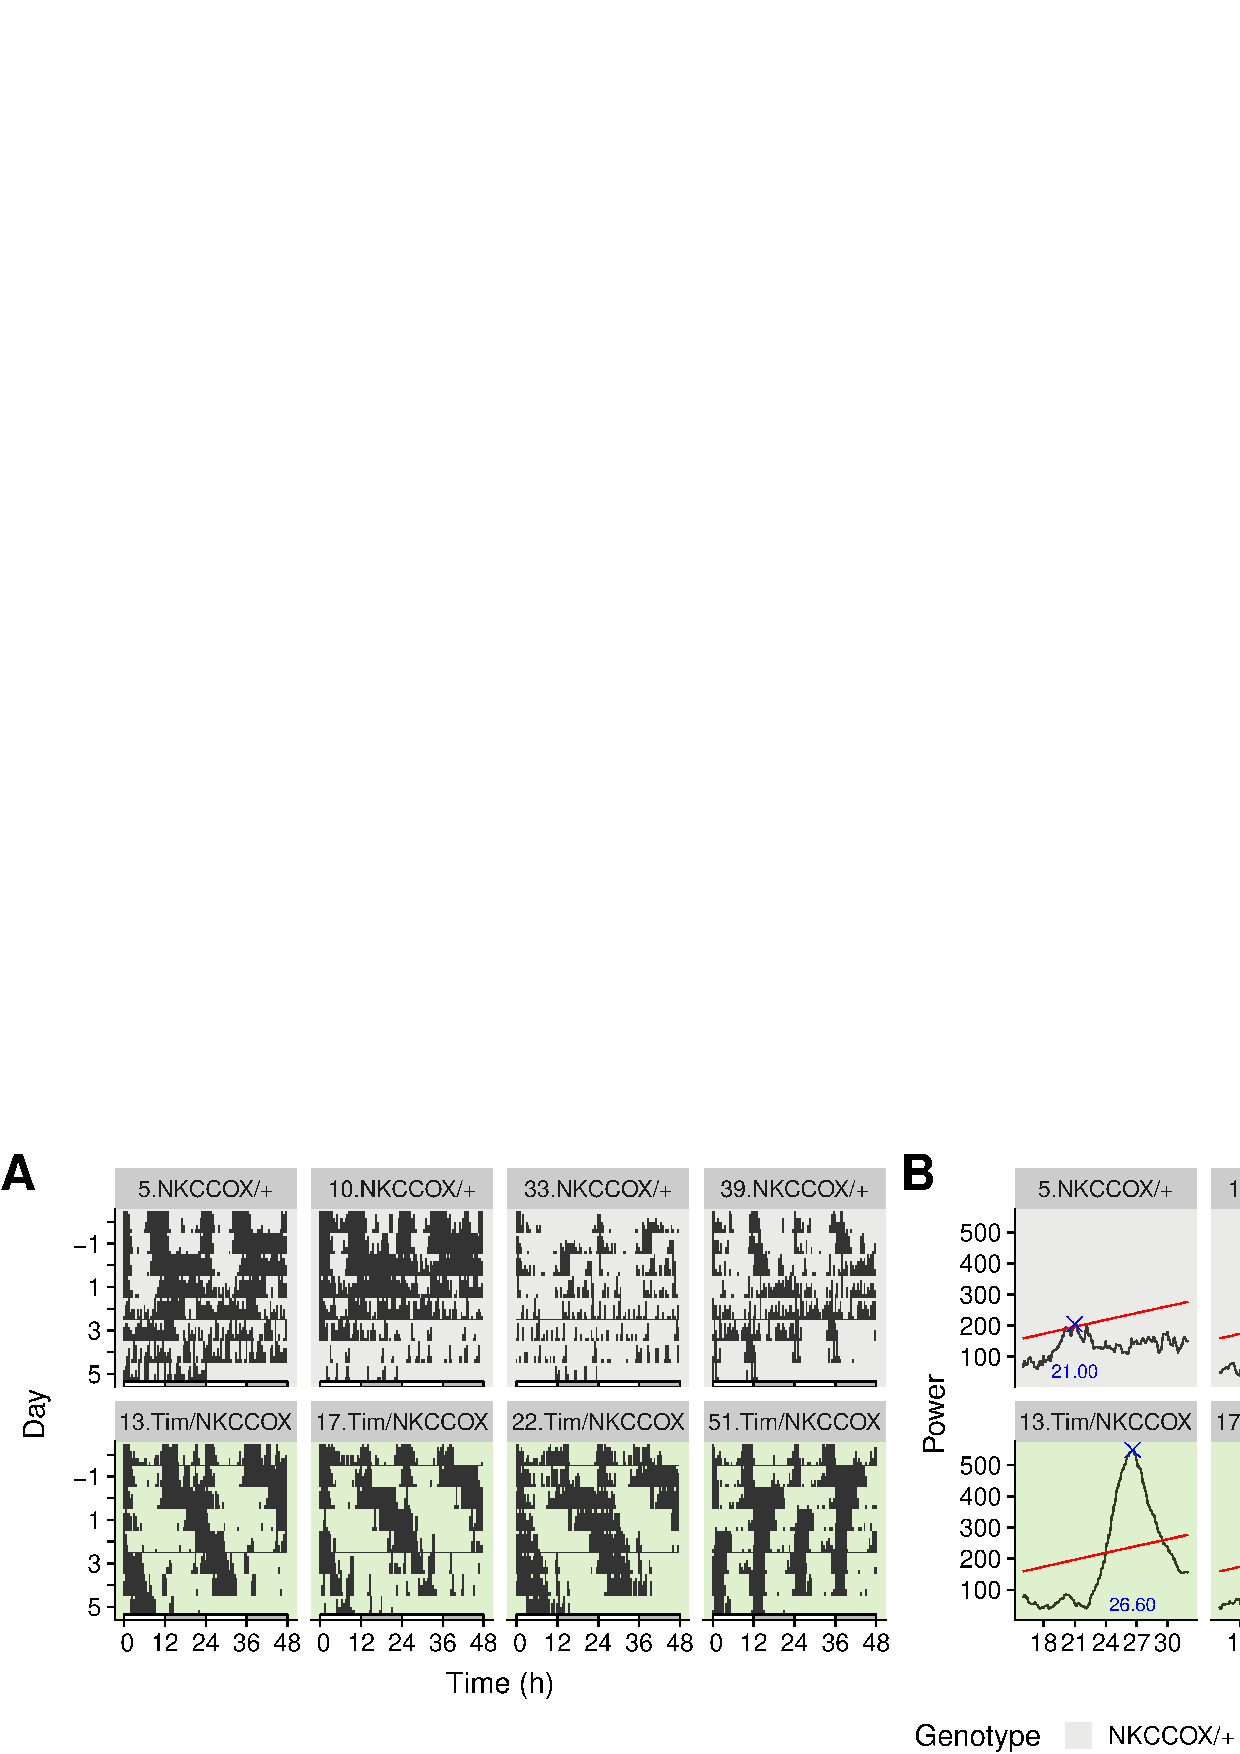
\includegraphics[width=1\textwidth]{fig/fig-4.pdf}
	\caption{{\bf Visualisation of the periodicity in activity of eight representative animals.}
		A: Double-plotted actograms showing activity over the experiment. Transition from LD to LL happens at day 0.
		B: $\chi{}^2$ periodograms over the LL part of the experiment matching the animals in A.
		The blue cross represents the first peak (if present) above the significance threshold (red line).
		Titles on top of each facet refer to the label allocated to each individual.
		See \nameref{S1-Fig} for all 52 animals.
	}
	\label{fig:fig-4}
\end{figure}

\subsection*{Population statistics}

As shown in the original study, double-plotted actograms and periodograms suggest that NKCC\textsuperscript{ox}/+ flies are mostly 
arhythmic in LL whilst Tim/NKCC\textsuperscript{ox} appear to have a consistent, long-period rhythm.
To visualise this at the population scale, we can plot an average periodogram (see Fig~\ref{fig:fig-5}A):

\begin{knitrout}
\definecolor{shadecolor}{rgb}{0.969, 0.969, 0.969}\color{fgcolor}\begin{kframe}
\begin{alltt}
\hlcom{# display periodogram }
\hlstd{fig5A} \hlkwb{<-} \hlkwd{ggperio}\hlstd{(per_dt,} \hlkwd{aes}\hlstd{(}\hlkwc{y} \hlstd{= power} \hlopt{-} \hlstd{signif_threshold,}
                             \hlkwc{colour} \hlstd{= genotype))} \hlopt{+}
          \hlcom{# periododogram shown as a line for population mean}
          \hlcom{# and bootstrap error bars}
          \hlkwd{stat_pop_etho}\hlstd{(}\hlkwc{method} \hlstd{= ggplot2}\hlopt{::}\hlstd{mean_cl_boot)} \hlopt{+}
          \hlcom{# rename x and y axis }
          \hlkwd{scale_y_continuous}\hlstd{(}\hlkwc{name} \hlstd{=} \hlstr{"Relative power"}\hlstd{)} \hlopt{+}
          \hlkwd{scale_x_hours}\hlstd{(}\hlstr{"Period"}\hlstd{)}
\end{alltt}
\end{kframe}
\end{knitrout}



\begin{figure}[!h]
%  	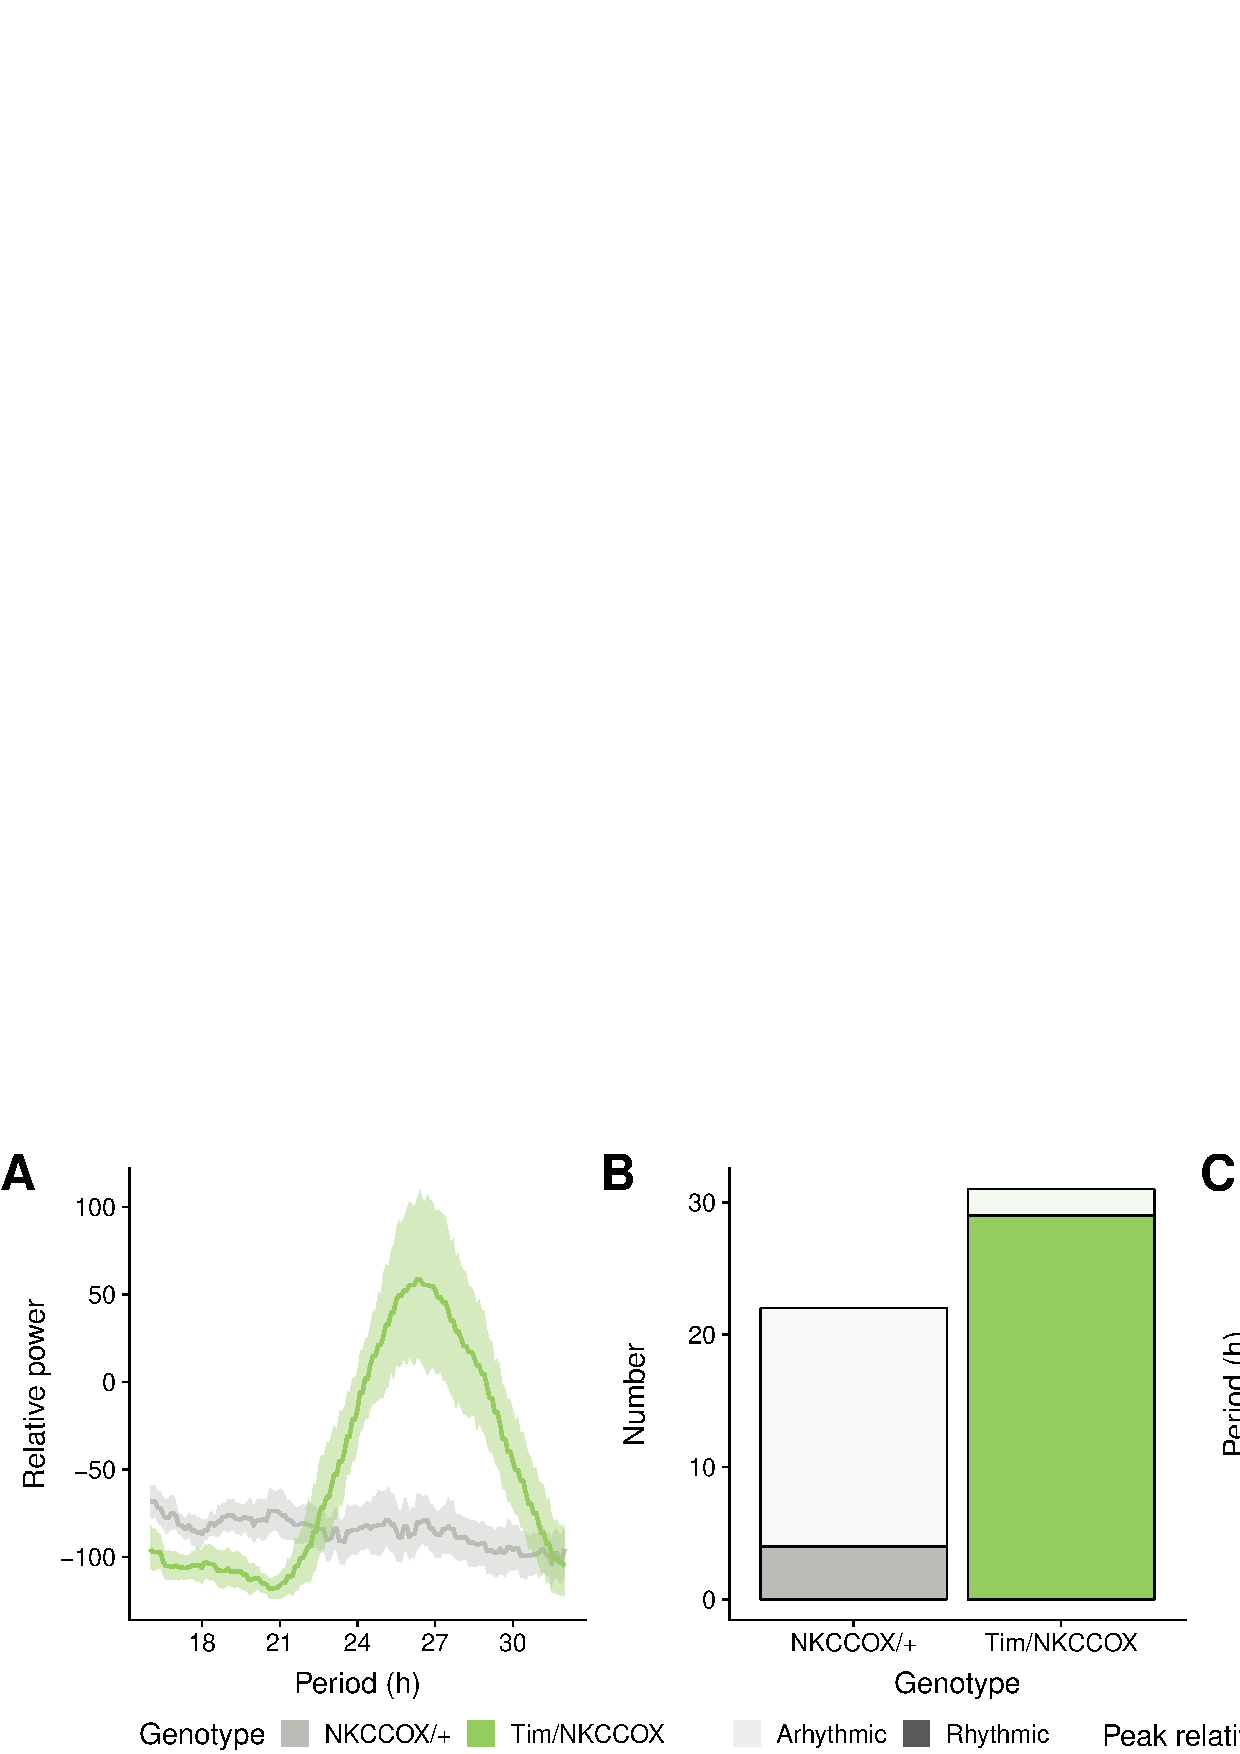
\includegraphics[width=1\textwidth]{fig/fig-5.pdf}
	\caption{{\bf Population statistics on circadian phenotype.}
			A: Average periodograms. 
			      The aggregated relative power of the periodogram of all animals.
			      The solid lines and the shaded areas show population means and their 95\% bootstrap confidence interval, respectively.
			B: Frequencies of rhythmic animals.
			      Number of rhythmic animals (\emph{i.e.} with a significant peak) in each genotypes.
			      Dark and clear fillings indicate rhythmic and arhythmic animals, respectively.
      C: Peak periodicity power and average.
			      Values of the peak period for animals with a significant peak (\emph{i.e.} rhythmic).
			      Individual animals are shown by dots whose size represent relative power of the peak period.
			      The error bars are 95\% bootstrap confidence interval on the population mean.
			      }
	\label{fig:fig-5}
\end{figure}


To further quantify this difference, we can show the number of rhythmic animals -- \emph{i.e.} individuals for which a peak was found -- in each group (see Fig~\ref{fig:fig-5}B).
Then, we can compare the average value of the peak for the rhythmic animals (see Fig~\ref{fig:fig-5}C).
First of all, we compute a summary per individual (\texttt{by=id}):

\begin{knitrout}
\definecolor{shadecolor}{rgb}{0.969, 0.969, 0.969}\color{fgcolor}\begin{kframe}
\begin{alltt}
\hlstd{summary_dt} \hlkwb{<-}
    \hlstd{per_dt[,}
          \hlkwd{.}\hlstd{(}
           \hlkwc{first_peak_period} \hlstd{= period[peak} \hlopt{==} \hlnum{1}\hlstd{],}
            \hlcom{# \{\} can be used for tmp variables}
           \hlkwc{first_peak_rel_power} \hlstd{= \{}
             \hlstd{signif} \hlkwb{=} \hlstd{signif_threshold[peak} \hlopt{==} \hlnum{1}\hlstd{]}
             \hlstd{power} \hlkwb{=} \hlstd{power[peak} \hlopt{==} \hlnum{1}\hlstd{]}
             \hlstd{power} \hlopt{-} \hlstd{signif}
            \hlstd{\},}
           \hlkwc{is_rhythmic} \hlstd{=} \hlkwd{any}\hlstd{(peak} \hlopt{==} \hlnum{1}\hlstd{)}
           \hlstd{),}
           \hlkwc{by}\hlstd{=id]}

\hlcom{# rejoin metadata}
\hlstd{summary_dt} \hlkwb{<-} \hlkwd{rejoin}\hlstd{(summary_dt)}
\end{alltt}
\end{kframe}
\end{knitrout}

\texttt{summary\_dt} is just a regular data frame with one row per individual, containing both metadata and our summary statistics. It can therefore be used directly by \texttt{ggplot} and other tools:

\begin{knitrout}
\definecolor{shadecolor}{rgb}{0.969, 0.969, 0.969}\color{fgcolor}\begin{kframe}
\begin{alltt}
\hlcom{# standard ggplot}
\hlstd{fig5B} \hlkwb{<-} \hlkwd{ggplot}\hlstd{(summary_dt,} \hlkwd{aes}\hlstd{(}\hlkwc{x} \hlstd{= genotype,}
                                \hlkwc{fill} \hlstd{= genotype,}
                                \hlkwc{alpha} \hlstd{= is_rhythmic}
                                \hlstd{))} \hlopt{+}
              \hlkwd{geom_bar}\hlstd{(}\hlkwc{colour}\hlstd{=}\hlstr{"black"}\hlstd{)}
\end{alltt}
\end{kframe}
\end{knitrout}

\begin{knitrout}
\definecolor{shadecolor}{rgb}{0.969, 0.969, 0.969}\color{fgcolor}\begin{kframe}
\begin{alltt}
\hlcom{# standard ggplot}
\hlstd{fig5C} \hlkwb{<-} \hlkwd{ggplot}\hlstd{(summary_dt,} \hlkwd{aes}\hlstd{(}\hlkwc{y} \hlstd{= first_peak_period,}
                                \hlkwc{x} \hlstd{= genotype))} \hlopt{+}
              \hlcom{# draw the mean of each genotype group}
              \hlkwd{stat_summary}\hlstd{(}\hlkwc{fun.y} \hlstd{= mean,} \hlkwc{geom} \hlstd{=} \hlstr{"point"}\hlstd{,} \hlkwc{shape}\hlstd{=}\hlnum{3}\hlstd{)} \hlopt{+}
              \hlcom{# draw bootstrap confidence intervals}
              \hlkwd{stat_summary}\hlstd{(}\hlkwc{fun.data} \hlstd{= mean_cl_boot,} \hlkwc{geom} \hlstd{=} \hlstr{"errorbar"}\hlstd{)} \hlopt{+}
              \hlcom{# shows all individuals as points}
              \hlcom{# the size of the point expresses the power of the peak}
              \hlkwd{geom_jitter}\hlstd{(}\hlkwd{aes}\hlstd{(}\hlkwc{colour} \hlstd{= genotype,}
                              \hlkwc{size} \hlstd{= first_peak_rel_power),}
                              \hlkwc{alpha} \hlstd{=} \hlnum{0.67}\hlstd{)} \hlopt{+}
              \hlcom{# We would like to convert time in hour}
              \hlkwd{scale_y_hours}\hlstd{(}\hlstr{"Period"}\hlstd{)}
\end{alltt}
\end{kframe}
\end{knitrout}


\texttt{R} provides one of the richest statistical toolbox available, which allows users to go deeper in the analysis of the extracted variables.
One could, for instance, perform a $\chi{}^2$ test on the number of rhythmic \emph{vs} arhythmic flies in both genotypes.
To address the same question, we fit a binomial generalised linear model:

\begin{knitrout}
\definecolor{shadecolor}{rgb}{0.969, 0.969, 0.969}\color{fgcolor}\begin{kframe}
\begin{alltt}
\hlstd{fit} \hlkwb{<-} \hlkwd{glm}\hlstd{(is_rhythmic} \hlopt{~} \hlstd{genotype, summary_dt,} \hlkwc{family} \hlstd{=} \hlstr{"binomial"}\hlstd{)}

\hlkwd{summary}\hlstd{(fit)}\hlopt{$}\hlstd{coefficients}
\end{alltt}
\begin{verbatim}
##                     Estimate Std. Error   z value     Pr(>|z|)
## (Intercept)        -1.504077  0.5527708 -2.720978 6.508902e-03
## genotypeTim/NKCCOX  4.143135  0.9172057  4.517127 6.268433e-06
\end{verbatim}
\end{kframe}
\end{knitrout}



The result shows a strong positive effect of genotype Tim/NKCC\textsuperscript{ox} on the probability of being rhythmic ($p$-value $6.27 \times 10^{-06}$):

Lastly, we can generate a table that compute arbitrary population statistics for each genotype:
\begin{knitrout}
\definecolor{shadecolor}{rgb}{0.969, 0.969, 0.969}\color{fgcolor}\begin{kframe}
\begin{alltt}
\hlstd{result_dt} \hlkwb{<-} \hlstd{summary_dt[,}
          \hlkwd{.}\hlstd{(}
            \hlkwc{mean_period} \hlstd{=} \hlkwd{mean}\hlstd{(first_peak_period,} \hlkwc{na.rm} \hlstd{= T)} \hlopt{/} \hlkwd{hours}\hlstd{(}\hlnum{1}\hlstd{),}
            \hlkwc{sd_period} \hlstd{=} \hlkwd{sd}\hlstd{(first_peak_period,} \hlkwc{na.rm} \hlstd{= T)} \hlopt{/} \hlkwd{hours}\hlstd{(}\hlnum{1}\hlstd{),}
            \hlkwc{n_rhythmic} \hlstd{=} \hlkwd{sum}\hlstd{(is_rhythmic),}
            \hlkwc{n} \hlstd{= .N,}
            \hlkwc{percent_rhythmic} \hlstd{=} \hlnum{100} \hlopt{*} \hlkwd{sum}\hlstd{(is_rhythmic)} \hlopt{/} \hlstd{.N}
            \hlstd{),}
          \hlkwc{by} \hlstd{= genotype}
          \hlstd{]}
\hlstd{result_dt}
\end{alltt}
\begin{verbatim}
##      genotype mean_period sd_period n_rhythmic  n percent_rhythmic
## 1:   NKCCOX/+    25.22500  3.598495          4 22         18.18182
## 2: Tim/NKCCOX    26.21429  2.363568         28 30         93.33333
\end{verbatim}
\end{kframe}
\end{knitrout}

This example shows how \texttt{rethomics} can be used from the raw data to making publication-quality figures and statistics.
We were able to comprehensively analyse the data from a circadian experiment with a few line of code.
This workflow applies particularly to much larger data sets and provides a large degree of flexibility that will allow biologists to tune their analysis to their specific questions.



% We present an small example examining the circadian behaviour of 128 fruit flies in recorded in a DAM2 -- a paradigm very widely adopted. 
% A less formal description of this case and others are explained at \href{https://rethomics.github.io/}{https://rethomics.github.io/}.
% In order to prodive a more comprehensive and didactic example, data was altered and simplified.	
% Fig~\ref{fig:experiment} describes our case experiment (A) and the corresponding metadata (B).
% Briefly, three monitors were used each containing 16 males and 16 females of a different genotype (A, B and C).
% Two replicates were performed at different times.
% raw data and metadata files are publicly available TODO cite zenodo
% 

\section*{Availability and Future Directions}
All packages in the \texttt{rethomics} framework are available under the terms of the GPLv3 license and listed at
\href{https://github.com/rethomics}{https://github.com/rethomics/}.
Extensive installation instructions as well as reproducible demos and tutorials are available at
\href{https://rethomics.github.io/}{https://rethomics.github.io/}.
All packages are continuously integrated and unit tested on several version of \texttt{R} to minimise the risk of present and future issues.

Several users, in different research groups, have already adopted and are contributing to the future development framework.
Several new packages in the \texttt{rethomics} framework are currently envisaged. 
They include utilities to input new behaviour tracking methods and analyse position and multi-animal interactions.

\section*{Supporting information}

% Include only the SI item label in the paragraph heading. Use the \nameref{label} command to cite SI items in the text.
\paragraph*{S1 Fig.}
\label{S1-Fig}
{\bf Complete version of Fig~\ref{fig:fig-4}.}
See Fig~\ref{fig:fig-4} for legend.


\section*{Acknowledgements}
We would like to thank people who have directly or indirectly contributed to the this manuscript.
In particular, Han Kim, for his invaluable comments on the early versions of \texttt{rethomics} and his dedicated contribution to the tutorials.
Maite Ogueta, for making the results data available.
\TODO{@esteban names of the BA users}
Alice French, Hannah Jones and Diana Bicazan for their comments as early users.
Marcus Gosh, for his feed back on the manuscript.
Brenna Williams, for her help to support multi-beam DAMS.
Patrick Kr{\"a}tschmer, for his time discussing the conceptual framework.
\TODO{@giorgio do you think it is ok to thank Rob?} Robert Dickinson, for his support.


% Include only the SI item label in the paragraph heading. Use the \nameref{label} command to cite SI items in the text.
%\paragraph*{S1 Fig.}
%\label{S1_Fig}
%{\bf Bold the title sentence.} Add descriptive text after the title of the item (optional).

\nolinenumbers

% Either type in your references using
% \begin{thebibliography}{}
% \bibitem{}
% Text
% \end{thebibliography}
%
% or
%
% Compile your BiBTeX database using our plos2015.bst
% style file and paste the contents of your .bbl file
% here. See http://journals.plos.org/plosone/s/latex for 
% step-by-step instructions.
% 



\bibliography{manuscript}{}


%\begin{thebibliography}{10}
%\end{thebibliography}



\end{document}

